\newpage
\subsection{Caso d'uso UC3:  Registrazione utente }
\label{UC3}
\begin{figure}[ht]
	\centering
	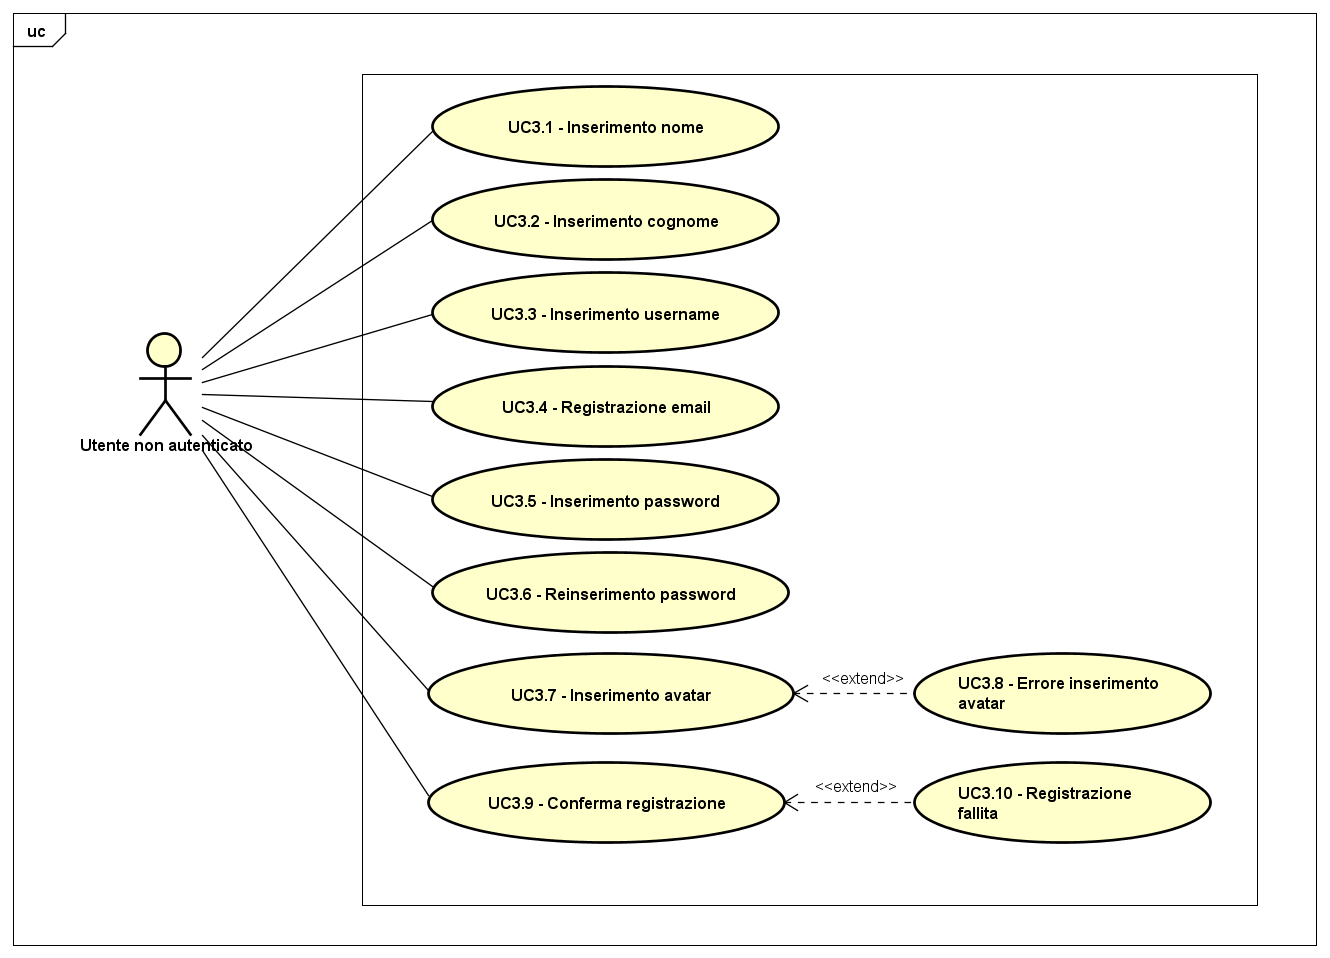
\includegraphics[scale=0.45]{UML/UC3.png}
	\caption{UC3: Registrazione utente}
\end{figure}

\begin{longtable}{ l | p{11cm}}
	\hline
	\rowcolor{Gray}
	 \multicolumn{2}{c}{UC3 - Registrazione utente} \\
	 \hline
	\textbf{Attori} & Utente non autenticato \\
	\textbf{Descrizione} & L'attore inserisce le sue informazioni personali per potersi registrare all'applicazione web, così da poter successivamente effettuare il login ed evolversi in un utente autenticato.
	L'amministratore API Market, oltre alle funzionalità offerte all'utente autenticato, può
	visualizzare i dati di utilizzo delle API ed amministrare l'applicazione web.  \\
	\textbf{Pre-Condizioni} & L'attore ha scelto di registrarsi e l'applicazione web mostra la schermata di registrazione \\
	\textbf{Post-Condizioni} & L'attore si è registrato all'applicazione web \\
	\textbf{Scenario Principale} & \begin{enumerate*}[label=(\arabic*.),itemjoin={\newline}]
		\item L'attore può inserire il proprio nome (UC3.1)
		\item L'attore può inserire il proprio cognome (UC3.2)
		\item L'attore può inserire il proprio username (UC3.3)
		\item L'attore può inserire la propria email (UC3.4) 
		\item L'attore può inserire la propria password (UC3.5)
		\item L'attore può reinserire la propria password per conferma (UC3.6)
		\item L'attore può confermare i dati inseriti, registrandosi all'applicazione web (UC3.7)
	\end{enumerate*}\\
\end{longtable}